\documentclass{beamer}
\usepackage[utf8]{inputenc}
\usepackage[T1]{fontenc}
\usepackage{lmodern}  % AMS mathematical facilities for LaTeX.
\usepackage{amsthm}   % Typesetting theorems (AMS style).
\usepackage{amsfonts} % 
\usepackage{mathrsfs}
\usepackage{amsmath,fourier}
\usepackage{amssymb}
\usepackage{cancel}
\usepackage{graphicx}
\usepackage{epsfig}
\usepackage{amsmath,amsfonts,amssymb}
\usepackage{mathpazo}
\usepackage{mathtools}
\theoremstyle{remark}
\newtheorem{remark}{Remark}
\theoremstyle{plain}
\newtheorem{proposition}{Proposition}
\theoremstyle{plain}
\usetheme{Berlin} % Choose a theme (e.g., Madrid, Berlin, etc.)
\usecolortheme{default} % Choose a color theme (e.g., default, albatross, etc.)

% Customize the title page
\title[Spin-0 fields NP constants]{The cylinder at spatial infinity and asymptotic charges}
\author[Rafael Pinto]{Rafael Pinto}
\institute[CENTRA-GRIT]{Instituto Superior Técnico}
\date{\today}
% Add a logo to the title page (optional)
\titlegraphic{
\vspace{-15mm}
\includegraphics[width=1.5cm]{centra.png}
\hspace{\fill}

\includegraphics[width=1.5cm]{grit.png}
}

\begin{document}

% Title Page
\begin{frame}
  \titlepage
  \vfill
  \begin{center}
    Advisors: \textbf{Dr. Edgar Gasper\'in} and \textbf{Dr. Alex Va\~{n}\'o Vi\~{n}uales}
  \end{center}
\end{frame}

% Table of Contents (optional)
\begin{frame}{Table of Contents}
  \tableofcontents
\end{frame}

% Section 1: Introduction
\section{Newman-Penrose constants}
\begin{frame}{Introduction}
  \begin{itemize}
    \item The Newman-Penrose (NP) constants serve as conserved quantities at null infinity in asymptotically flat gravitational fields.
    \item These constants present a comprehensive conservation system for various spins: spin-1 fields and spin-2 fields, with our research focusing on spin-0 fields linked to wave equation solutions.
    \item In the detailed context, while an infinite series of conserved quantities is identified in the linear theory, the non-linear General Relativity theory conserves only ten.
  \end{itemize}
\end{frame}

\begin{frame}{Conservation laws}
  \begin{itemize}
    \item These charges are computed as 2-surface integrals at cuts ${C} \approx \mathbb{S}^2$ of null infinity $\mathscr{I}$.
  \end{itemize}
  \begin{figure}[h]
    \centering 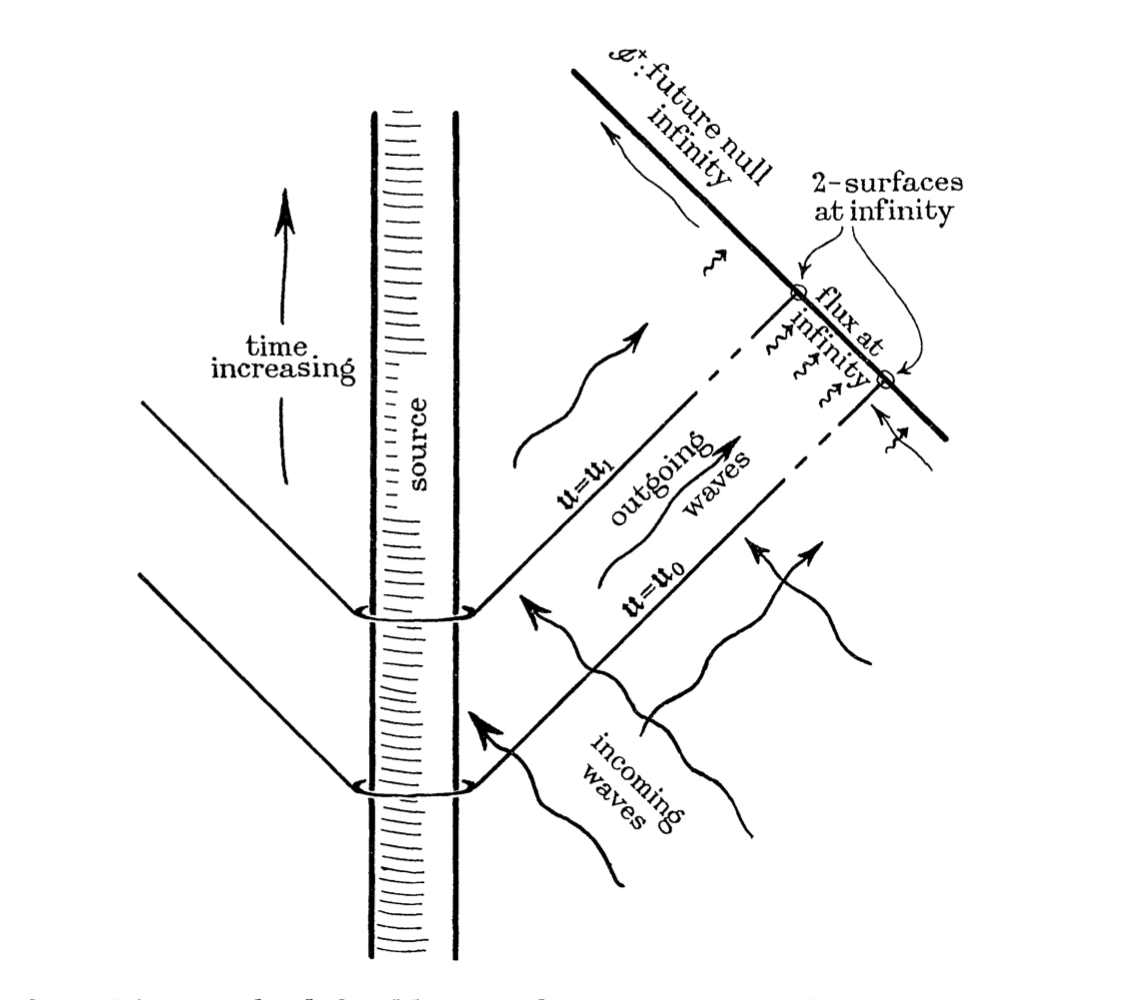
\includegraphics[width =0.45\textwidth]{penrose constants.png}
      \caption{Visual representation of the behavior of the Newman-Penrose constants at null infinity.}
  \end{figure}
\end{frame}

\begin{frame}{Spin-1 (EM) Field}
  \begin{itemize}
    \item A complex tetrad can be selected as follows:
      \begin{align}\label{eq:tetrad}
        & l^{\mu} = \delta_{1}^{\mu}, \quad n^{\mu} = \delta_{0}^{\mu} - \delta_{1}^{\mu}, \nonumber \\
        & m^{\mu} = \displaystyle\frac{1}{\tau}\left(\delta_{2}^{\mu} + \displaystyle\frac{1}{\sin\theta}\ \delta_{3}^{\mu}\right), \qquad \overline{m}^{\mu} = \displaystyle\frac{1}{\tau}\left(\delta_{2}^{\mu} - \displaystyle\frac{1}{\sin\theta}\ \delta_{3}^{\mu}\right).
      \end{align}
    \item To describe the electromagnetic (EM) field, we make use of three complex tetrad components of the Maxwell field tensor denoted as $F_{\mu \nu}$:
      \begin{align}\label{eq:Maxtensor}
        & \Phi_{0} = F_{\mu \nu}l^{\mu}n^{\nu}, \nonumber \\
        & \Phi_{1} = \frac{1}{2} F_{\mu \nu}(l^{\mu}n^{\nu} + \overline{m}^{\mu}m^{\nu}), \nonumber \\
        & \Phi_{2} = F_{\mu \nu}\overline{m}^{\mu}n^{\nu}.
      \end{align}
  \end{itemize}
\end{frame}

\begin{frame}{NP Constants Calculation}
  \begin{itemize}
    \item The NP constants are calculated using the following formula:
    \begin{equation}
      F_{m}^{n,k} = \int{_{1}\overline{Y}_{n-k+1,m}\Phi_{0}^{n+1} d\omega}.
    \end{equation}
    \item The interpretation of charges, such as the Newman-Penrose constants, remains an open debate, yet their conservation is evident in general asymptotically flat spacetimes, even in events like black hole collisions.
  \end{itemize}
\end{frame}
% Section 2: Literature Review
\section{Cylinder at $i^0$}
\begin{frame}{The $i^0$ cylinder representation in Minkowski  spacetime}
  \begin{itemize}
    \item Consider spherical polar coordinates $(\tilde{t}, \tilde{\rho}, \vartheta^A)$
    with $A = 1, 2$.
    \item The metric of physical Minkowski spacetime in this coordinate system is given by $\tilde{\boldsymbol{\eta}}$:
    \begin{equation}
      \tilde{\boldsymbol{\eta}}=-\mathbf{d} \tilde{t} \otimes \mathbf{d} \tilde{t}+\mathbf{d} \tilde{\rho} \otimes \mathbf{d} \tilde{\rho}+\tilde{\rho}^2 \boldsymbol{\sigma}.
    \end{equation}
    \item Introduce unphysical spherical polar coordinates $(t, \rho, \vartheta^A)$ as an intermediate step:
    \begin{equation}
      t = \frac{\tilde{t}}{\tilde{\rho}^2 - \tilde{t}^2}, \quad \rho = \frac{\tilde{\rho}}{\tilde{\rho}^2 - \tilde{t}^2}.
    \end{equation}
    \item The conformal metric in unphysical coordinates, $\boldsymbol{\eta} = \Xi^2 \boldsymbol{\tilde{\eta}}$: 
    \begin{equation}
      \boldsymbol{\eta} = -\frac{1}{\tilde{\rho}^2 - \tilde{t}^2} (-\mathbf{d} \tilde{t} \otimes \mathbf{d} \tilde{t} + \mathbf{d} \tilde{\rho} \otimes \mathbf{d} \tilde{\rho} + \tilde{\rho}^2 \boldsymbol{\sigma}).
    \end{equation}
  \end{itemize}
\end{frame}

\begin{frame}
  \frametitle{$i^0$ Representation in Unphysical Coordinates}
  \begin{itemize}
    \item In this conformal representation ($t \in (-\infty, \infty)$, $\rho \in [0, \infty)$), spatial infinity and the origin interchange.
    \item $i^0$ is represented by the point $(t = 0, \rho = 0)$ in $(\mathbb{R}^4, \eta)$.
    \item Introduce coordinates $(\tau, \rho, \vartheta^A)$ with $t = \rho \tau$.
    \item Consider the conformal metric $\boldsymbol{g} = \rho^{-2} \boldsymbol{\eta}$.
    \item Express the unphysical metric $\boldsymbol{g}$ in $F$-coordinates:
    \begin{align}
      & \boldsymbol{g} = -\mathbf{d} \tau \otimes \mathbf{d} \tau + \frac{1 - \tau^2}{\rho^2} \mathbf{d} \rho \otimes \mathbf{d} \rho - \frac{\tau}{\rho} \left(\mathbf{d} \rho \otimes \mathbf{d} \tau + \mathbf{d} \rho \otimes \mathbf{d} \tau\right) + \boldsymbol{\sigma}.
    \end{align}
  \end{itemize}
\end{frame}

\begin{frame}
  \frametitle{Conformal Factor and Lorentz Transformation}
  \begin{itemize}
    \item The conformal factor $\Theta$ in $F$-coordinates and physical coordinates:
    \begin{align}
      \Theta := \rho (1-\tau^2) = \frac{1}{\tilde{\rho}}.
    \end{align}
    \item The boost parameter $\kappa$:
    \begin{align}
      \kappa := \frac{1+\tau}{1-\tau} = -\frac{\tilde{v}}{\tilde{u}}.
    \end{align}
    \item The Lorentz transformation that connects the NP and F-frames:
    \begin{align}
      (\Lambda_{+})^{2} := \Theta^{-1}\kappa^{-1}, \quad (\Lambda_{-})^{2} := \Theta^{-1}\kappa.
    \end{align}
  \end{itemize}
\end{frame}

\begin{frame}
  \frametitle{$i^0$ Cylinder and Null Frames}
  \begin{itemize}
    \item Identify future and past null infinity in the conformal representation:
    \begin{align*}
      \mathscr{I}^{+} & \equiv \{ p \in \mathcal{M} \; \rvert\; \tau(p) =1\}, \\
      \mathscr{I}^{-} & \equiv \{ p \in \mathcal{M} \; \rvert \;\tau(p) =-1\}.
    \end{align*}
    \item The $i^0$-cylinder represents spatial infinity as an extended set $I \approx \mathbb{R}\times \mathbb{S}^2$:
    \begin{align*}
      I & \equiv \{ p \in \mathcal{M} \; \rvert \;\; |\tau(p)| < 1, \;\rho(p)=0\}, \\
      I^{0} & \equiv \{ p \in \mathcal{M}\; \rvert \;\tau(p)=0, \; \rho(p)=0\}.
    \end{align*}
  \end{itemize}
\end{frame}

\begin{frame}
  \frametitle{$F$-Frame and Null Frames}
  \begin{itemize}
    \item Introduce the $F$-frame:
    \begin{align}
      & \boldsymbol{e}=(1+\tau) \boldsymbol{\partial}_\tau-\rho \boldsymbol{\partial}_\rho, \quad \underline{\boldsymbol{e}}=(1-\tau) \boldsymbol{\partial}_\tau+\rho \boldsymbol{\partial}_\rho, \quad \boldsymbol{e}_{\boldsymbol{A}} \quad \text { with } \nonumber \\ 
      & \boldsymbol{A}=\{\uparrow, \downarrow\}.
    \end{align}
    \item The NP-frame hinged at $\mathscr{I}^{\pm}$:
    \begin{align*}
      \text{NP hinged at} \; \mathscr{I}^{+}: & \quad \boldsymbol{e}^{+}, \underline{\boldsymbol{e}}^{+}, \boldsymbol{e}_{\boldsymbol{A}}^{+}, \\
      \text{NP hinged at} \; \mathscr{I}^{-}: & \quad \boldsymbol{e}^{-}, \underline{\boldsymbol{e}}^{-}, \boldsymbol{e}_{\boldsymbol{A}}^{-}.
    \end{align*}
    \item Transformation between NP and F-frames:
    \begin{align*}
      \text{\emph{NP hinged at} $\mathscr{I}^{+}$}:& \quad\boldsymbol{e}^{+} = \Theta^{-2} L, \quad \underline{\boldsymbol{e}}^{+}= \underline{L},\quad \boldsymbol{e}_{\boldsymbol{A}}^{+}= \boldsymbol{e}_{\boldsymbol{A}}= \Theta^{-1}\tilde{\boldsymbol{e}}_{\boldsymbol{A}}\\ \text{\emph{NP hinged at} $\mathscr{I}^{-}$}:& \quad\boldsymbol{e}^{-} =
       L,\quad \underline{\boldsymbol{e}}^{-}=  \Theta^{-2} \underline{L},\quad \boldsymbol{e}_{\boldsymbol{A}}^{-}= \boldsymbol{e}_{\boldsymbol{A}} = \Theta^{-1}\tilde{\boldsymbol{e}}_{\boldsymbol{A}}.
    \end{align*}
  \end{itemize}
\end{frame}

% Section 3: Methodology
\section{Spin-0 fields close to $i^0$ and $\mathscr{I}$}
\begin{frame}{Spin-0 fields close to $i^0$ and $\mathscr{I}$}
  % Your content for the methodology goes here
\end{frame}

% Section 4: Results
\section{Results}
\begin{frame}{Results}
  % Your content for the results goes here
\end{frame}

% Section 5: Conclusion
\section{Conclusion}
\begin{frame}{Conclusion}
  % Your content for the conclusion goes here
\end{frame}

% References (optional)
\section{References}
\begin{frame}{References}
  % Your references go here
\end{frame}

% Thank You Slide
\begin{frame}{Thank You}
  % Thank your audience and any acknowledgments
\end{frame}

\end{document}
